% Titre : suites
% Filiere : BCPST
% Difficulte : 
% Type : TD 
% Categories :suites
% Subcategories : 
% Keywords : suites




\begin{exercice} \;
\'Etudier la suite $\suiteu$ d\'efinie par  $u_0\in \R$ et $\forall n \geq 1$, $u_{n+1}=e^{u_n}.$
%
%$\left\lbrace\begin{array}{l}
%u_0\in\R\vsec\\
%u_{n+1}=e^{u_n}.
%\end{array}\right.$
\end{exercice}


\%\%\%\%\%\%\%\%\%\%\%\%\%\%\%\%\%\%\%\%
\%\%\%\%\%\%\%\%\%\%\%\%\%\%\%\%\%\%\%\%
\%\%\%\%\%\%\%\%\%\%\%\%\%\%\%\%\%\%\%\%




\begin{correction} \;
C'est une suite de type $u_{n+1}=f(u_n)$, on donne les id\'ees de l'\'etude.
\begin{enumerate}
 \item \'Etude de la fonction $f$ associ\'ee: $x\mapsto e^x$\\
\noindent  La fonction $f$ est d\'efinie, continue et d\'erivable sur $\R$ et 
$$\forall x\in\R,\ f^{\prime}(x)=e^x.$$
On obtient ainsi le tableau de variation suivant:
\begin{center}
\begin{tikzpicture}
 \tkzTabInit{ $x$          /1,%
       %$f'(x)$      /,%
       $f(x)$       /2}%
     { $-\infty$ ,$+\infty$ }%
  \tkzTabVar{
       -/ $0$        /,
       +/$+\infty$           /,
                      } 
 \tkzTabVal[draw]{1}{2}{0.5}{$0$}{$1$}
\end{tikzpicture}
\end{center}
\item Calcul des limites \'eventuelles:\\
\noindent La fonction $f$ est continue sur $\R$, ainsi, si la suite $\suiteu$ converge, elle ne peut converger que vers $l$ v\'erifiant 
$l=f(l)$. 
\'Etudions alors la fonction $g:\ x\mapsto g(x)=f(x)-x$. L'\'etude d'une telle fonction donne que:
$$\forall x\in\R,\quad g(x)\geq 1.$$
En particulier, il n'y a pas de valeur d'annulation de $g$ et donc il n'y a pas de limite \'eventuelle pour la suite $\suiteu$.
\item La suite est bien d\'efinie et elle appartient \`{a} $I$ intervalle stable par $f$:\\
\noindent $\R^+$ est un intervalle stable par $f$ et $u_1>0$.
\noindent Ainsi, on montre par r\'ecurrence que la suite est bien d\'efinie et que : $\forall n\in\N^{\star},\quad u_n \geq 0$. (On ne commence pas au rang 0 car $u_0\in\R$).
\item \'Etude de la monotonie de la suite:\\
\noindent Soit $n\in\N$, on a: $u_{n+1}-u_n=g(u_n)\geq 1>0$. Donc la suite $\suiteu$ est croissante.
\item \'Etude de la convergence de la suite:\\
\noindent La suite $\suiteu$ est croissante donc d'apr\`es le th\'eor\`eme sur les suites monotones, elle tend vers une limite finie ou $+\infty$. Comme il n'y a pas de limite \'eventuelle possible, par un raisonnement par l'absurde, on obtient que la suite $\suiteu$ tend vers $+\infty$
\end{enumerate}
\end{correction}